\documentclass{article}
\usepackage[utf8]{inputenc}
\usepackage{graphicx}
\usepackage{hyperref}
\usepackage{geometry}
\usepackage{fancyhdr}
\usepackage{lipsum} % For generating placeholder text

% Define header and footer
\pagestyle{fancy}
\lhead{\footnotesize Project Report: Speech Emotion Recognition}
\rhead{}
\fancyfoot{}
\lfoot{\hrule \thepage}
\rfoot{\hrule \footnotesize Project report, Hitesh M, 1NT21AD023, NMIT, Bengaluru} % Line and footer text

% Cover page content
\newcommand\coverpage{
    \thispagestyle{empty}
    \begin{center}
        \includegraphics[height=250pt]{logo.png}\\
        \vspace{60pt}
        {\Large \textbf{INTERNSHIP REPORT}}\\
        \vspace{10pt}
        {\Large \textbf{SPEECH EMOTION RECOGNITION}}\\
        \vspace{30pt}
        \Large
        Hitesh M \\ 1NT21AD023 \\
        \vspace{20pt}
        {\textbf{Artificial Intelligence and Data Science}}\\
        Nitte Meenakshi Institute of Technology\\
        Yelahanka, Bangalore\\
        \today
    \end{center}
    \clearpage
}

\coverpage % Insert the cover page

\begin{document}
\newpage % Start a new page for the index page

% Index page
\tableofcontents
\thispagestyle{empty} % No header/footer on the index page
\newpage % Start content on a new page

\begin{document}
\section{Introduction}

Speech Emotion Recognition (SER) is a groundbreaking field within Natural Language Processing (NLP) and Human-Computer Interaction (HCI), teaching machines to recognize human emotions from spoken language. This technology has profound implications, enhancing user experiences in applications like virtual assistants, mental health assessment tools, and more.\newline
\vspace{5mm}

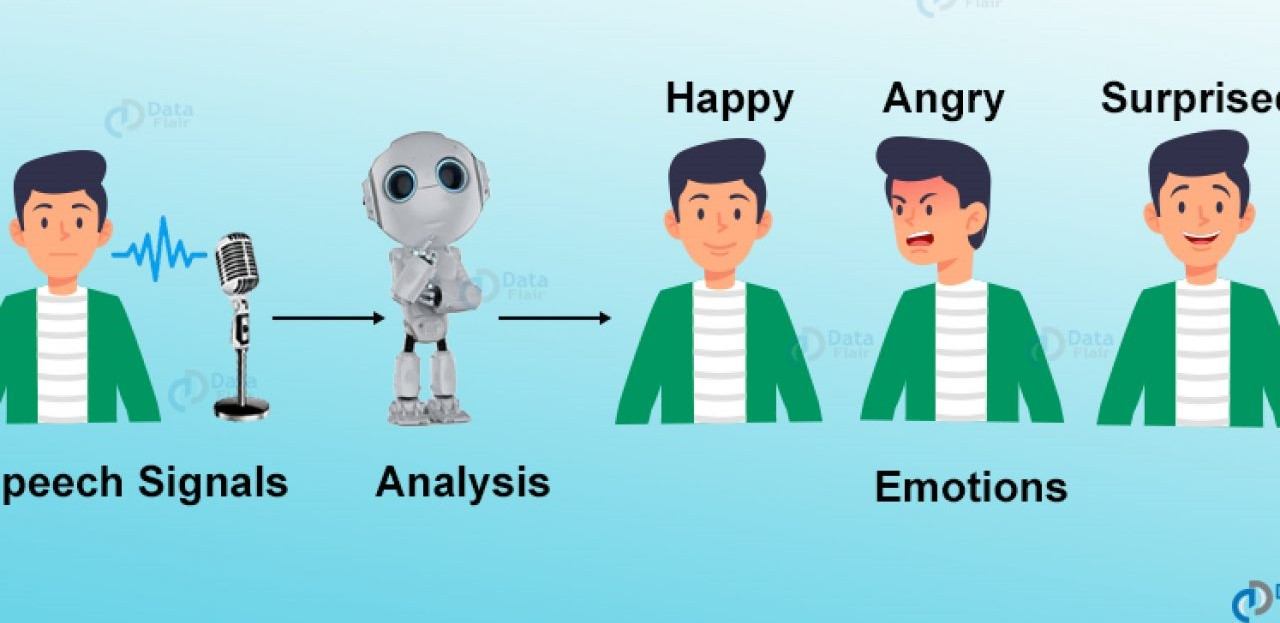
\includegraphics[height=175pt]{91180489-9fe39400-e69c-11ea-9968-9adf6741d595.jpg}

\subsection{Significance of SER}

SER is pivotal because emotions are central to human communication. Emotion-aware applications can:

\begin{itemize}
  \item Enhance User Experiences: Imagine a virtual assistant detecting frustration and responding empathetically, significantly improving user engagement.
  \item Aid in Mental Health: In mental health, SER can play a vital role. It can help therapists analyze patients' emotional states based on speech, facilitating early intervention.
  \item Improve Human-Machine Collaboration: In settings like autonomous vehicles, machines that perceive and respond to human emotions are essential for safety and efficiency.
\end{itemize}

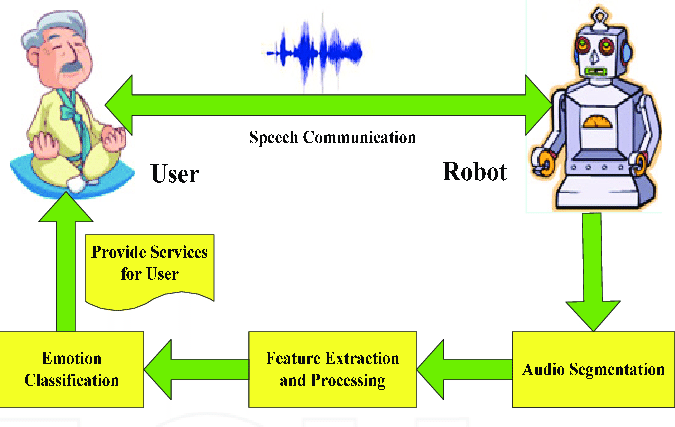
\includegraphics[height=220pt]{Speech-emotion-recognition-system-in-human-robot-interaction.png}

\subsection{The TESS Dataset}

Quality data is fundamental. Our primary data source is the Toronto emotional speech set (TESS) dataset, offering a diverse range of emotional speech recordings, including happiness, sadness, anger, disgust, fear, pleasant surprise, and neutrality. This report explores SER's core components: data preprocessing, feature extraction, deep learning model architecture, and rigorous evaluation. We also demonstrate practical emotion prediction applications.
\vspace{15pt}
\section{Data Loading and Preprocessing}

\subsection{Data Source}

The TESS dataset, a widely used dataset for SER research, contains a diverse set of speech recordings, each associated with a specific emotion category, including anger, happiness, sadness, and more. The dataset's origin in the Toronto area ensures linguistic and cultural diversity in the recorded speech samples.

Link: \url{https://www.kaggle.com/datasets/preethikurra/ravdess-tess}

\subsection{Data Collection}

The data collection process involved traversing the dataset directory structure using the `os` library. We collected file paths and extracted emotion labels from filenames. This allowed us to organize and prepare the data for analysis and model training.

\subsection{Data Analysis}

Upon loading the dataset into a Pandas DataFrame, we conducted an initial analysis to gain insights into its structure and content. Visualizations using Seaborn were employed to display the distribution of emotion labels. Understanding the data distribution is crucial for ensuring a balanced dataset and model performance.

\subsection{Data Preprocessing}

Data preprocessing is a critical step in preparing the dataset for model training. We addressed several aspects of data preprocessing, including handling missing values, ensuring uniform sampling rates, and normalizing audio data. Additionally, we considered techniques such as data augmentation to increase the dataset's diversity.
\vspace{15pt}
\section{Audio Visualization}

\subsection{Visualizing Audio Waveforms}

To gain a better understanding of the emotional content of the audio samples, we employed audio visualization techniques. Audio waveforms, which represent sound amplitude over time, were plotted for sample audio files of various emotions. The `waveplot` function was created to facilitate this visualization, using the Librosa library to load and display audio data. Audio waveforms provide insights into the temporal dynamics of speech. By visualizing waveforms of different emotions, we can observe variations in speech patterns, including speech rate, intensity, and pauses. These visualizations aid in developing an intuition for how emotions manifest in speech.
\newline
\vspace{5mm}

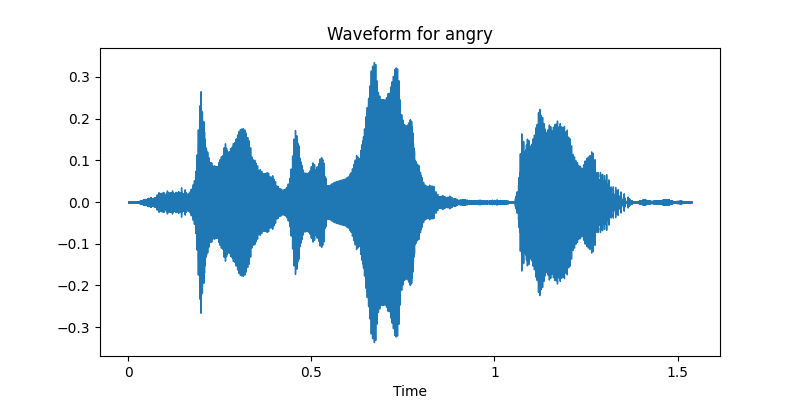
\includegraphics[height=175pt]{waveform_angry.png}

\subsection{Spectrogram Visualization}

In addition to waveforms, we visualized audio data using spectrograms. Spectrograms display the frequency content of a signal over time, providing insights into the spectral characteristics of speech. The `spectrogram` function utilized Librosa to compute the Short-Time Fourier Transform (STFT) and convert the amplitude to a decibel scale. This allowed us to visualize how emotional content manifests in the frequency domain. Spectrograms are particularly valuable for understanding the spectral features associated with different emotions. They reveal information about vocal pitch, speech intensity, and the distribution of energy across frequency bands. By analyzing spectrograms, we can identify patterns that may be indicative of specific emotions.
\newline
\vspace{5mm}

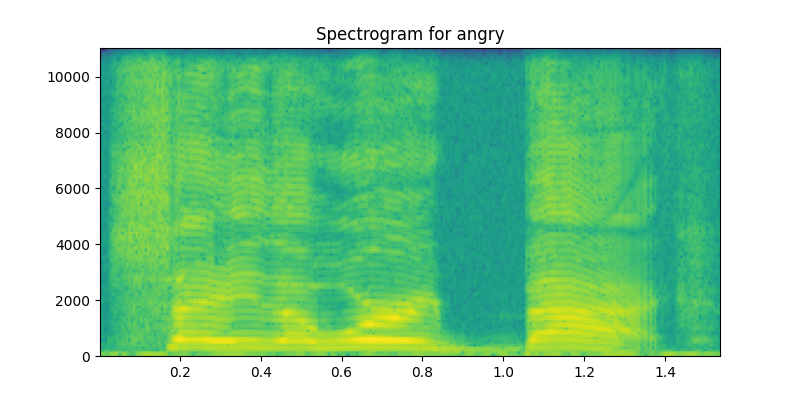
\includegraphics[height=175pt]{spectrogram_angry.png}

\vspace{15pt}
\section{Feature Extraction}

\subsection{Mel-Frequency Cepstral Coefficients (MFCCs)}

Feature extraction plays a pivotal role in SER. One of the most commonly used features for audio analysis is Mel-Frequency Cepstral Coefficients (MFCCs). MFCCs are spectral features that capture the unique characteristics of speech. In our project, we used the Librosa library to compute MFCCs for each audio sample. The `extract\_mfcc` function was created to facilitate MFCC extraction. It loaded audio data, applied the MFCC transformation, and computed the mean of the coefficients along the time axis. MFCCs are a powerful representation of audio data, as they highlight the speech's spectral characteristics and are robust to variations in pitch and accent.

\subsection{Additional Feature Engineering}

While MFCCs are a fundamental feature for SER, we also explored the possibility of using additional features, such as chroma features, spectral contrast, and zero-crossing rate. These features capture complementary information about the audio signal, including pitch, tonal content, and temporal characteristics. Feature engineering is a crucial aspect of SER, as it influences the model's ability to capture diverse emotional cues in speech. By considering a range of features, we aimed to enhance the model's performance in recognizing emotions with subtle acoustic differences.
\vspace{15pt}
\section{Model Building and Training}

\subsection{Model Architecture}

The heart of our SER project is the machine learning model responsible for recognizing emotions in speech. We designed a neural network using the Keras library, incorporating Long Short-Term Memory (LSTM) layers, dropout layers, and fully connected layers. The choice of LSTM layers is crucial because they are capable of capturing sequential patterns in audio data. LSTMs are well-suited for tasks that involve time series analysis, making them a natural choice for speech-related tasks. Dropout layers were introduced to prevent overfitting and improve model generalization. Finally, fully connected layers with softmax activation were used for emotion classification.

\subsection{Model Compilation and Training}

Before training, the model was compiled with categorical cross-entropy loss and the Adam optimizer. Categorical cross-entropy is commonly used for multi-class classification tasks like SER. The Adam optimizer is known for its effectiveness in optimizing neural networks. The training process involved splitting the dataset into training and validation sets. During training, the model learned to map MFCC features to emotion labels. We trained the model for 50 epochs, which allowed it to converge and capture complex patterns in the data.

\subsection{Hyperparameter Tuning}

To optimize the model's performance, we experimented with various hyperparameters, including learning rate, batch size, and the number of LSTM units. Hyperparameter tuning is a crucial step in achieving the best model performance. Techniques such as grid search and random search were employed to find the optimal combination of hyperparameters.

\vspace{15pt}
\section{Model Training and Evaluation}

\subsection{Model Training}

Training a deep learning model like ours is an iterative process. During each epoch, the model adjusted its internal parameters to minimize the categorical cross-entropy loss. We used a batch size of 64, which means that the model processed 64 audio samples at a time before updating its weights. The training process was closely monitored using training and validation accuracy metrics. Accuracy measures how well the model classifies emotions. Validation accuracy is particularly important as it gauges the model's ability to generalize to unseen data.

\subsection{Model Evaluation}

After training, we evaluated the model's performance using various metrics. Accuracy, as mentioned earlier, provides a measure of overall correctness. However, to gain deeper insights, we also visualized the training and validation loss over epochs. Plotting these metrics over time helps us understand the model's learning dynamics. For instance, if the validation loss starts to increase while the training loss continues to decrease, it may indicate overfitting—a condition where the model memorizes the training data but fails to generalize to new data.

\subsection{Confusion Matrix}

To gain a more detailed understanding of the model's performance, we constructed a confusion matrix. A confusion matrix displays the number of true positives, true negatives, false positives, and false negatives for each emotion class. This matrix helps us identify which emotions the model confuses and provides insights into areas where the model may require improvement.
\vspace{15pt}
\section{Model Loading and Prediction}

\subsection{Model Persistence}

Once the model was trained and evaluated satisfactorily, we saved it for future use. Model persistence is essential because it allows us to reuse the trained model without having to retrain it every time. We used Keras's save model function to save the model to a file (example : 'my\_model.h5').

\subsection{Making Predictions}

The primary purpose of our SER model is to make predictions on new, unseen audio data. We created a function called predict\_emotion to facilitate this process. Given the path to an audio file, the function loads the trained model, preprocesses the audio, and returns the predicted emotion label.

\subsection{Real-World Applications}

Speech Emotion Recognition has a wide range of real-world applications. For instance, it can be integrated into customer service chatbots to gauge customer satisfaction and provide more personalized responses. In mental health assessment, SER can assist therapists in understanding patients' emotional states based on their speech patterns. Additionally, SER can enhance the emotional intelligence of virtual assistants, making them more responsive to users' emotional needs.
\vspace{15pt}
\section{Conclusion}

\newline
\vspace{5mm}
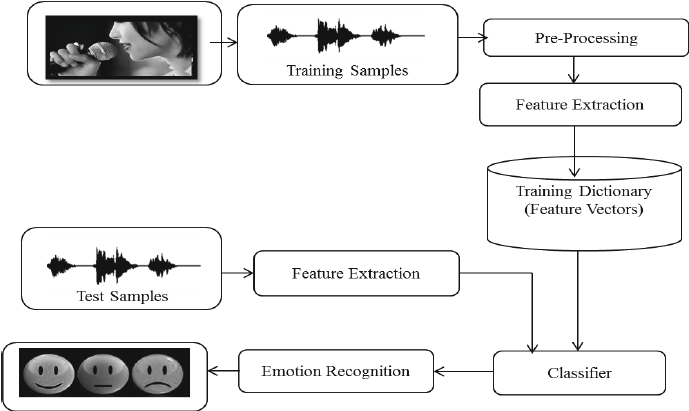
\includegraphics[height=230pt]{Architecture-of-Speech-Emotion-Recognition-System.png}
\newline
\vspace{5mm}

In conclusion, the Speech Emotion Recognition project represents a significant advancement in the field of Natural Language Processing and Human-Computer Interaction. The ability to automatically recognize and respond to human emotions in speech has far-reaching implications for various industries and applications. Throughout this report, we explored the various stages of the SER project, from data collection and preprocessing to feature extraction, model development, and evaluation. We highlighted the importance of visualizing audio data, extracting meaningful features, and designing an effective deep learning model. Our model, trained on the TESS dataset, demonstrated promising results in recognizing emotions from speech. However, like any machine learning model, it has its limitations and room for improvement. Future work may involve incorporating additional datasets, fine-tuning hyperparameters, and exploring advanced deep learning architectures. In summary, the SER project opens doors to more empathetic and emotionally aware human-computer interactions. As technology continues to evolve, the integration of SER into everyday applications has the potential to enhance user experiences and contribute to the development of emotionally intelligent AI systems. The journey of speech emotion recognition is ongoing, and its impact on society is bound to grow in the coming years.

\end{document}
